\documentclass[12pt, a4paper]{article}
\usepackage{setspace}
%\onehalfspacing
\setstretch{1.2}


\usepackage{graphicx} % Required for inserting images
\usepackage{subcaption}  % Wichtig für nebeneinander + Untertitel
\usepackage[utf8]{inputenc}
\usepackage[ngerman]{babel}  %, ngerman]
\usepackage{mathtools}
\usepackage{relsize}
\usepackage[left=2cm, right=2cm, top=2.5cm, bottom=2.5cm]{geometry}
\graphicspath{{images/}}
\usepackage[inkscapeformat=png]{svg}
\usepackage[version=4]{mhchem}
\usepackage{multirow}
\usepackage{makecell}
\usepackage{siunitx}
%\usepackage[dvipsnames]{xcolor}
%\usepackage{hyperref}
\usepackage{booktabs}
\usepackage{fancyvrb}
\usepackage{enumitem}
\usepackage{fancyhdr}
\usepackage{xcolor,tikz, tcolorbox}
\usepackage{siunitx}
\usepackage{float}

\usepackage[backend=biber,style=numeric,sorting=none]{biblatex}
%\usepackage[style=apa, backend=biber,sorting=ynt]{biblatex}
%\DeclareLanguageMapping{english}{english-apa}
\addbibresource{references.bib}
%\bibliography{Referenzen1}

\setlength{\parindent}{15pt}
\setlength{\parskip}{0.3\baselineskip}

\title{FOPRA - Electron spectroscopy of surfaces}
\author{Alex Greck, Boyan Totev}
\date{01.09.2025}

\begin{document}

\maketitle
\tableofcontents

\newpage

\section{Einleitung}

\section{Theoretische Grundlagen}
\subsection{Stickstoff-Fehlstellen-Zentren in Diamant}
Stickstoff-Fehlstellen-Zentren sind Defektstellen in einer kristalinen Diamantstruktur, welche aus einer direkten Nachbarschaft einer Leerstelle und eines P1-Zentrums gebildet werden. Ein P1-Zentrum ist eine Defektstelle bestehend aus einem einzigen Stickstoff-Donator. Im neutralen Zustand enthält das NV (an der Fehlstelle) fünf Elektronen, wobei 3 von den angrenzenden Kohlenstoffatomen herrühren und zwei weitere vom benachbarten Stickstoff. In der Praxis relevant sind aber s.g. NV$^-$-Zentren welche ein zusätzliches Elektron aus dem Kristall aufnehmen und somit eine negative Ladung besitzen. Betrachtet man für die sechs-Elektron Konfiguration das Tight-Binding Modell und die Orbitalbesetzung stellt man fest, dass NV$^-$
einen Gesamtspin von S=1 zu eigen haben und sowohl ein elektronischer Grundzustand $^3A_2$ als auch ein angeregter Zustand $^3E$ existieren. Außerdem können die Elektronenspins antiparallel zu einem Gesamtspin von S=1 koppeln. Üblicherweise spricht man von Singulet (S=0) und Triplet (S=1) Konfigurationen. Liegt zudem ein äußeres Magnetfeld an, spalten sich die Triplett-Zustände durch den Zeeman-Effekt in drei Feinstruktur-Niveaus auf, welche mit magnetischen Quantenzahlen $m_S$ nummeriert werden. Einen Überblick über die Level-Struktur von NV$^-$-Zentren liefert Abbildung \ref{fig:level structure}.

\begin{figure}
    \centering
    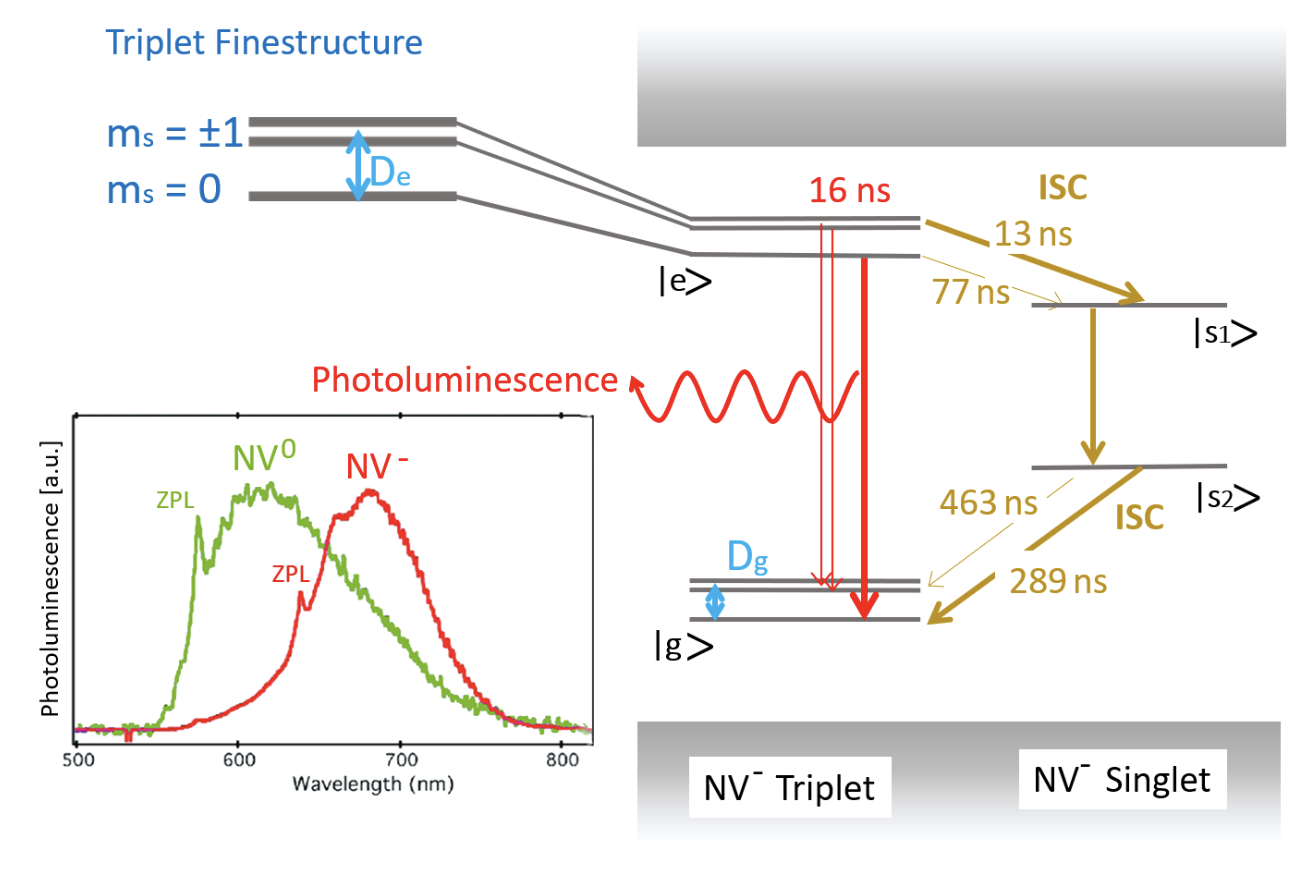
\includegraphics[width=0.8\linewidth]{Level structure.png}
    \caption{Level-Struktur für ein NV$^-$-Zentrum in Diamant.}
    \label{fig:level structure}
\end{figure}

Allerdings ist ein Spinsystem allein völlig unpraktisch, insofern es nicht initialisiert, manipuliert und anschließend wieder ausgelesen werden kann. Diese Schritte erfolgen in diesem Praktikum durch optisches Pumpen mit grünem ($\lambda_{in} = ??$) Laserlicht. Dadurch wird das NV-Zentrum vom Grundzustand in den nächst höheren Zustand angeregt. Nun sind zwei verschiedene Prozesse möglich:
\begin{itemize}
    \item Gewöhliche Relaxation: Zum einen kann das NV-Zentrum gewöhnlich relaxieren ohne die Quantenzahlen $S$ und $m_S$ zu verändern. Nach dem Frank-Condon-Prinzip ändert sich aber die Wellenlänge des emittierten Lichts. Die gemessene Photoluminescence beträgt üblicherweise eine Wellenlänge von $637\,\si{nm}$ (rotes Licht).
    \item Inter-System-Crossing: Ein dazu konkurrierender Effekt ist das Inter-System-Crossing. Dabei untergeht das NV-Zentrum einen vermeindlich Spin-verbotenen Übergang vom Triplet zum Singulet Zustand. Dieser Übergang ist im sichtbaren Bereich nicht strahlend. Bemerkenswert ist hierbei, dass dabei auch ein Wechsel der magnetischen Quantenzahl von $m_s=1$ zu $m_s=0$ zu beobachten ist. Wie meistens in quantenmechanischen Prozessen git dies nur statistisch für den Erwartungswert abhängig von Übergangsraten.
\end{itemize}

Durch diese Zentrale Eigenschaft lässt sich nun ein Ensemble aus NV$^-$-Zentren initialisieren indem durch optisches Pumpen der $m_s=0$ Zustand bevölkert wird.

Nach oder während eines Messung lässt sich auch der Endzustand des Ensembles auslesen, da sich durch Manipulation und Spin-Flips die Intensität der Photolumineszens ändert. Von dieser Helligkeitsänderung aus lässt sich auf den Besetzungszustand zurückschließen. 

\subsection{Hamilton Operator und Verhalten im Magnetfeld}
\subsection{Spindynamik und Darstellung auf der Blochkugel}

\section{Experimenteller Ablauf}
\subsection{Experimenteller Aufbau}
\subsection{CW-ODMR-Messung}
Im ersten Teil des Experiments wird eine einfache CW-ODMR-Messung durchgeführt. Dabei wird ein gewisser Frequenzbereich der Radiowellenstrahlung durchlaufen und parallel die Photolumineszenz der Probe gemessen. Dadurch lassen sich die Reonanzfrequenzen zur jeweiligen Umgebungssituation ermitteln. Diese sind durch Dips im Photolumineszensspektrum ersichtlich. Zunächst wird eine Messung ohne externes Magnetfeld durchgeführt, anschließend wird ein Feld mit einem kleinen Permanentmagneten angelegt und die Messung wiederholt.

\subsection{Rabi Sequenz}
Für die Rabi Sequenz wird nun die gemessene Resonanzfrequenz aus der CW-ODMR Messung genutzt, wobei diese gepulst und in verschiedenen Zeitlängen auf den Diamanten angelegt. 
\subsection{Hahn-Echo Sequenz}
\subsection{Ramsey Sequenz}

\section{Ergebnisse und Diskussion}
\subsection{CW ODMR Spektrum}
In einem ersten Schritt wurde die Resonanzfrequenz für Spin-Flips bestimmt. Für den Fall, dass kein äußeres Magnetfeld existiert muss diese dem Zero-Field-Splitting von $f_0=2,87\,\si{GHz}$ entsprechen. Daher wurde zunächst ohne angelegtes Magnetfeld eine CM-ODMR Messung im Bereich von $2,83$ -$2,93 \,\si{GHz}$ durchgeführt. Die Ergebnisse sind in Abbildung \ref{fig:ESR_ohne_Signal} dargestellt. Ein mit der Datenpunkte mit einer geeigneten Lorentzkurve ergeben eine experimentelle Resonanzfrequenz von $2.870\pm0.001 \,\si{GHz}$, was perfekt mit den theoretischen Erwartungen übereinstimmt. An dieser Stelle soll erwähnt werden, dass im Labor das externe Magnetfeld nicht völlig abgeschirmt werden konnte, sonder mindestens das Erdmagnetfeld vorhanden war. Dieses beträg in München ungefähr $50 \,\si{\mu T}$. Die Zemann-Aufspaltung der S=1 Niveaus ist proportional zu $28\,\si{GHz}$ pro Tesla. Setzt man die Werte ein, liefert das eine zu erwartende Abweichung von $1,4\,\si{MHz}$. Diese Abweichung ist so klein, dass sie praktisch nicht gemessen wird bzw. in der Unsicherheit verschwindet. Zudem beträgt der Spin-Kontrast (Baseline - Min. Dip) von -6.4\% auf. Die Halbwertsbreite wurde auf $9,62\pm0.18 \,\si{MHz}$ bestimmt. Diese ist in unserer experimentellen Umgebung haptsächlich von Temperatur, $^{13}\text{C}$ Konzentration sowie P1-Zentren Konzentration ($^{15}\text{N}$) und ggf. dem Power Broadening abhängig.

\begin{figure}[htbp]
    \centering
    % First Subfigure
    \begin{subfigure}[c]{0.49\textwidth}
        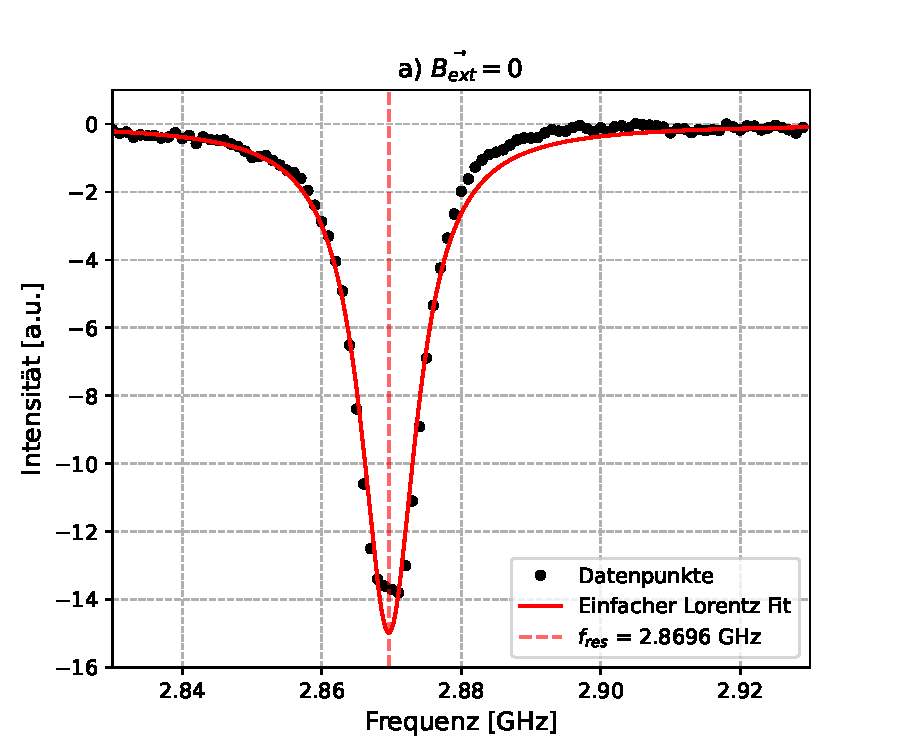
\includegraphics[width=\textwidth]{ESR ohne BFeld.pdf} % Best practice: no spaces in filename
        \caption{Ohne externes B-Feld} % Required for the label to work
        \label{fig:ESR_ohne_Signal}
    \end{subfigure}\hfill % \hfill pushes them apart, no blank lines here!
    % Second Subfigure
    \begin{subfigure}[c]{0.49\textwidth}
        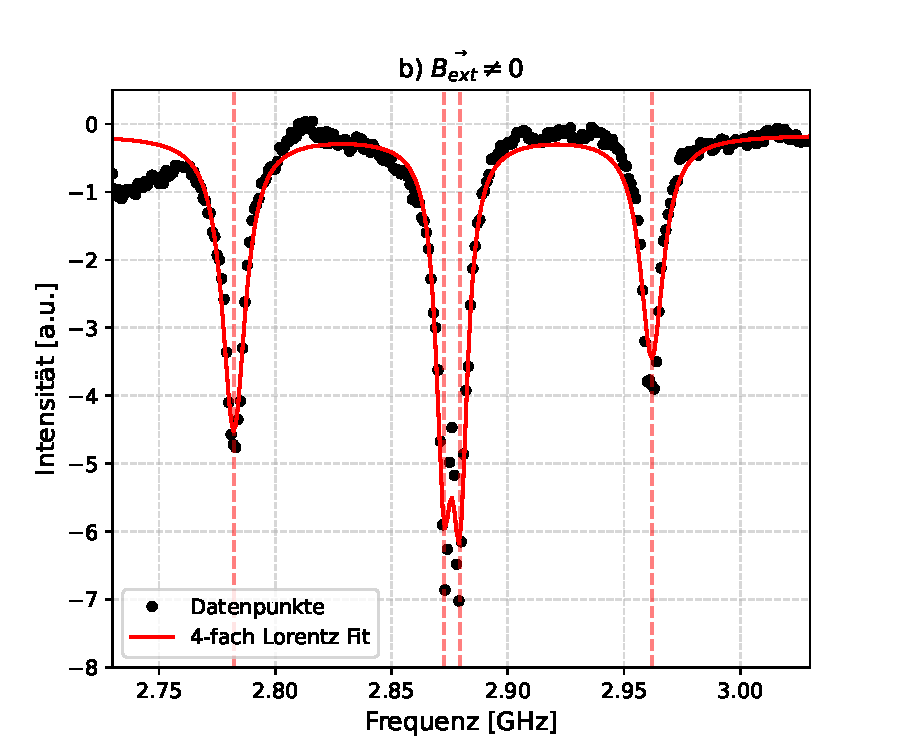
\includegraphics[width=\textwidth]{ESR mit BFeld.pdf}
        \caption{Mit externes B-Feld}
        \label{fig:ESR_mit_Signal}
    \end{subfigure}
    
    \caption{CW-ODMR-Messungen zur Bestimmung der Resonanzfrequenz ohne und mit angelegtem externen Magnetfeld.}
    \label{fig:ESR_Gesamt} % Optional: Added a label for the whole figure
\end{figure}
Anschließend wurde ein externes, statisches Magnetfeld in Form eines kleinen Permanentmagneten angelegt. Eine erneute CW-ODMR-Messung im Frequenzbereich von $2,73$ -$3,03 \,\si{GHz}$ liefert folgendes Bild \ref{fig:ESR_mit_Signal}. Wie unschwer zu erkennen ist, wurde der einzelne Dip für den magnetfeldfreien Fall in vier seperate Dips aufgespalten. Die Aufspaltung erfolgt dabei symmetrisch um $f_0$. Die beiden inneren Peaks sind um $3.5\pm0.3\,\si{MHz}$ verschoben und weist eine Dip-Tiefe von ca. 6 auf. Die äußeren Dips dahingegen haben sich um $90,0\pm0,2\,\si{MHz}$ im Vergleich zur vorherigen Messung nach außen bewegt. Die Diptiefe liegt dabei bei ca. 4.5 (links) und 3.5 (rechts). Die unterschiedlichen Intensitäten entsprechen dabei auch den Erwartungen. Wegen dem äußeren Magnetfeld lässt sich eine Vorzugsrichtugn im Diamant definieren. Für diese Messung relevant sind nun die Anteile, welche parallel zur Achse des NV-Zentrums liegen. Da in Diamant vier verschiedene Orientierungen vorliegen, können im CW-ODMR-Spektrum richtugnsabhängig bis zu acht Resonanzen festgestellt werden. Wählt man dagegen eine Magnetfeldrichtung parallel zu einer NV-Achse werden nur noch vier Dips beobachtet, wobei aus Symmetriegründen die innenren Dips die dreifache Intensität aufweisen sollten. Unsere Messungen bestätigen die Aufspaltung in vier Resonanzen mit jeweils paarweise unterschiedlichen Intensitäten, welche aber nicht ganz dem zu erwartenden Verhältnis von 1:3 entsprechen.

Ausgehend von diesen Überlegungen lässt sich das externe Magnetfeld abschätzen. Unter der Annahme, dass die äußeren Peaks einer parallelen Magnetfeldorientierung entsprechen ergibt sich mit Formel (\ref{}) eine Feldstärke von $3,2\,\si{mT}$. Dieses Resultat ist verhältnismäßig für einen kleinen Neodym-Permanentmagneten, mit welchem das externe Magnetfeld angelegt wurde.

\subsection{Rabi-Sequenz}
Für die Messung der Rabi-Sequenz wurde die kleinste Resonanzfrequenz aus der CW-ODMR Messung mit einer Frequenz von $f = \SI{2.785}{GHz}$ verwendet. Die gemessenen Daten sind in Abbildung \ref{fig:Rabi_0dB} dargestellt. Es ist ersichtlich, dass es sich hierbei um eine gedämpfte Kosinusschwingung handelt. Durch einen Fit erhält man eine Rabi-Frequenz von $f_R = \SI{1.05}{MHz}$ und eine Pi-Pulsdauer von $T_\pi = \SI{477}{ns}$.

\begin{figure}
    \centering
    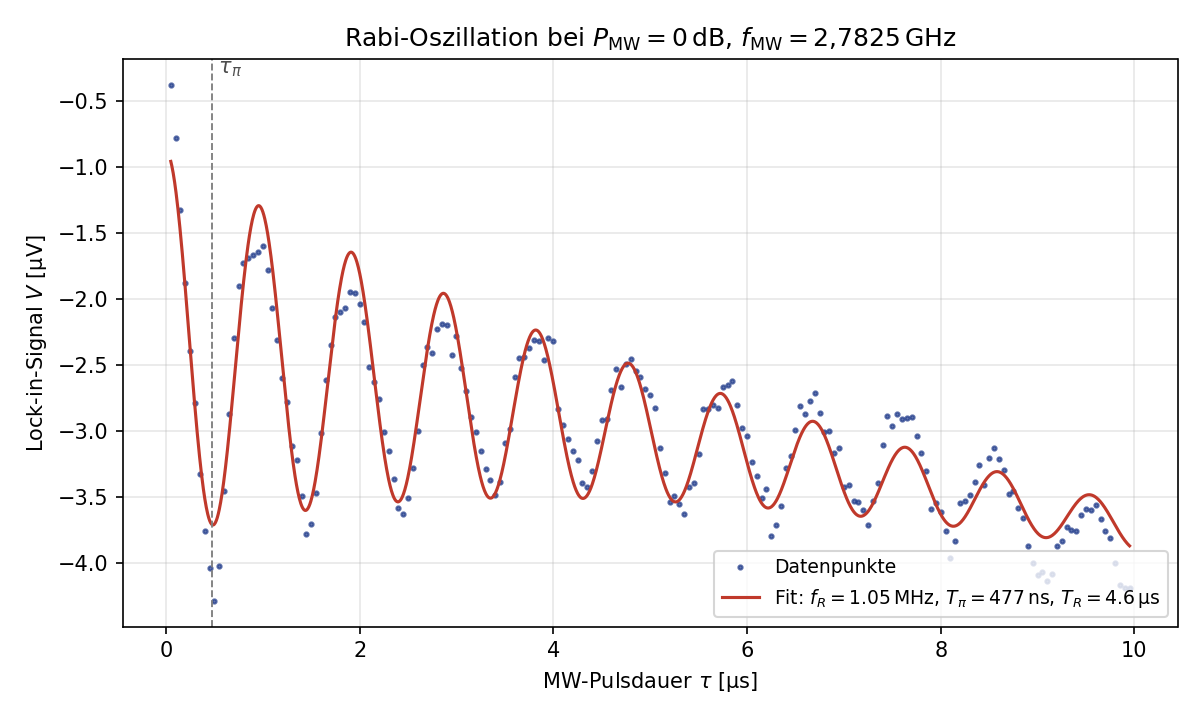
\includegraphics[width=0.9\linewidth]{Rabi_0dB.png}
    \caption{Rabi Sequenz für $P_\text{MW} = 0$ dB}
    \label{fig:Rabi_0dB}
\end{figure}
\subsection{Rabi-Sequenz: Zusatzaufgabe}

Es wird wieder die Resonanzfrequenz bei 2.785 GHz betrachtet. Diesmal wird die anregende 
Mikrowellenleistung von -13 dB bis 7 dB verändert. Die sich ergebenden Messungen sind in
Abbildung \ref{fig:Rabi-Zusatz} dargestellt. Für die Rabi-Frequenzen $f_R$ sowie die $\pi$-Pulsdauern $T_\pi$ ergibt sich:

\begin{figure}
    \centering
    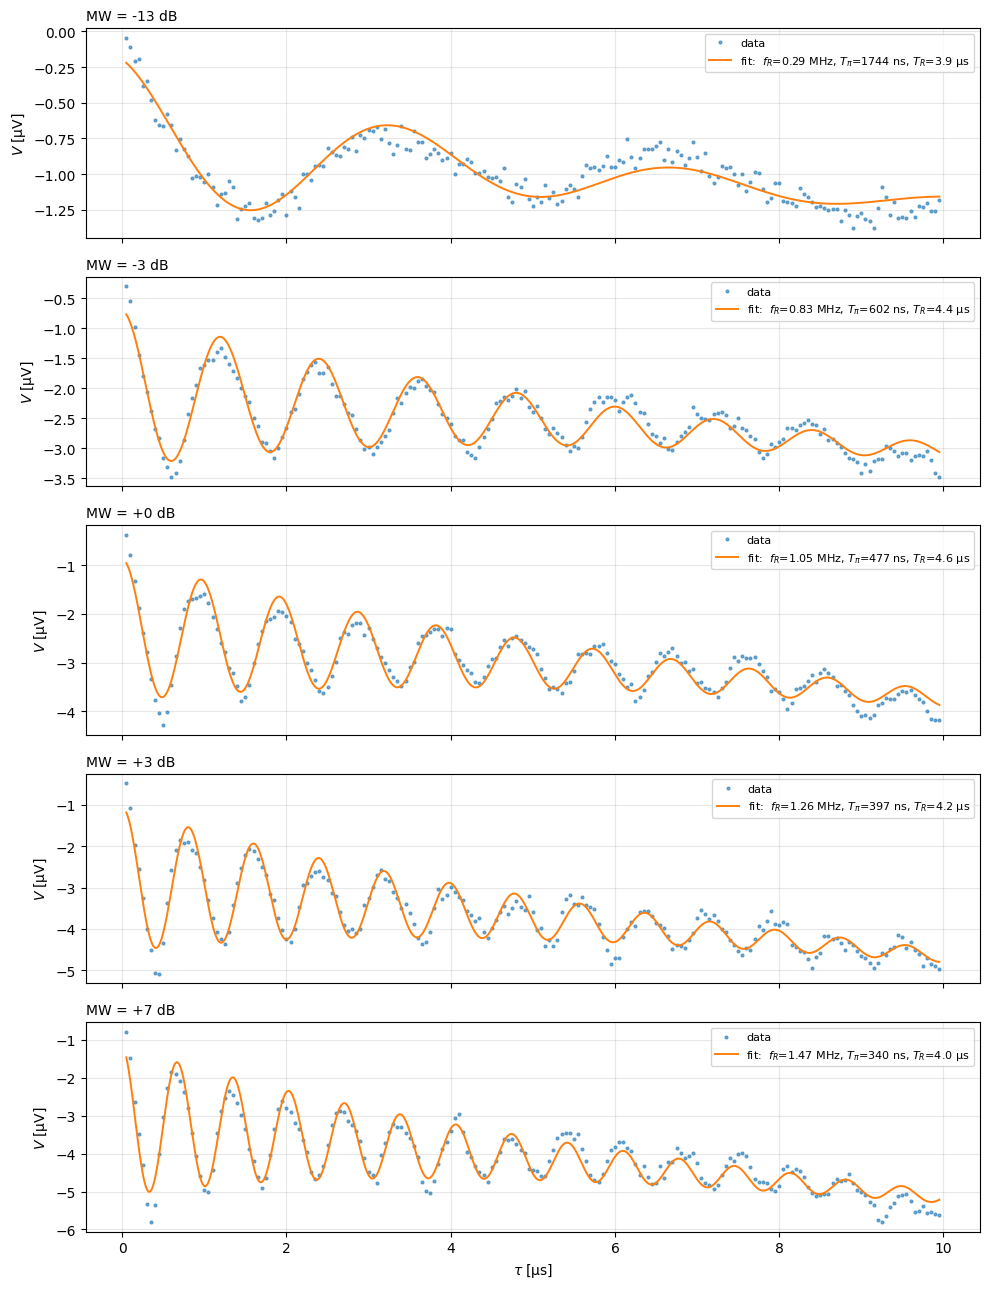
\includegraphics[width=1\linewidth]{Rabi_Zusatz.png}
    \caption{Rabi Sequenz mit verschiedenen Mikrowellenleistungen}
    \label{fig:Rabi-Zusatz}
\end{figure}
\end{document}